\scanpage{88}
\margin{87}
\mspage{- 24 -}

\uline{Preuve} : Soit $G$ un faisceau $C'$-acyclique. Il suffit de montrer que pour tout objet $X$ de $C$,
\[
\check H^q(C^{\wedge}/X,\mathcal H^0(u_{\unsure{s}}(G)))=0\qquad q>0
\]

Il suffit donc de montrer que pour toute famille couvrante
$\mathcal U=(U_i\longrightarrow X,\ i\in I)$ dont l'existence est assurée par la condition (\unsure{CWC|CNC}),
$H^q(\mathcal U,\mathcal H^0(u_{\unsure{s}}(G)))=0\quad\inserted{\forall}\ q>0$.
Mais $u$, étant un foncteur continu, transforme la famille couvrante $\mathcal U$ en une famille couvrante de $u(X)$ ; et par définition du foncteur image directe, on a l'égalité :
\[
H^q(\mathcal U,\mathcal H^0(u_{\unsure{s}}(G)))=H^q(u(\mathcal U),\mathcal H^0(G))
\]
\margin{$\unsure{\forall\ \longrightarrow}$}
Le faisceau $G$ étant $C'$-acyclique, ces groupes sont nuls pour tout $q>0$. c.q.f.d.

La notion de faisceau $C$-acyclique n'est pas intrinsèque.
Elle ne dépend pas uniquement du topos $C^{\sim}$ défini par le site $C$, mais aussi du site particulier choisi pour définir le topos $C^{\sim}$ (3.11).
Nous allons maintenant définir une propriété intrinsèque.

\margin{\figure{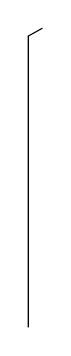
\begin{tikzpicture}[x=1cm,y=1cm]\draw (0.18,3.8)--(0,3.7)--(0,0);\end{tikzpicture}}}
\uline{Proposition 3.4} : Soient $E$ un topos annelé par un anneau $A$ de $E$, $F$ un $A$-Module. Les propriétés suivantes sont équivalentes :

i) Pour tout objet $S$ de $E$ :
\[
H^q(S,F)=0\qquad\inserted{\forall}\ q>0.
\]
\[\ldots/\ldots\]
